\documentclass[withoutpreface,bwprint]{cumcmthesis}

\usepackage[framemethod=TikZ]{mdframed}
\usepackage{url}
\usepackage{subcaption}
\usepackage{geometry}
\usepackage{ulem}
\usepackage{setspace}
\usepackage{array}
\usepackage{graphicx}
\usepackage{multirow}
\usepackage{hyperref}
\usepackage{amsmath}
\usepackage{amssymb}
\usepackage{bm}
\usepackage{longtable}
\usepackage{listings}
\usepackage{xcolor}

\graphicspath{{../q1_glrt_results/}{../q2_harmonic_recovery_results/}{../q3_multisource_separation_results_optimized_complete/}{../q4/figures/}{../../latex模板/figures/}}

\geometry{a4paper,left=25mm,right=25mm,top=25mm,bottom=25mm}
\title{基于广义似然比检验的机械设备微弱故障信号检测、恢复、分离与传感器布局优化}


\begin{document}
\xeCJKsetup{AutoFakeBold={2.5}}
\setCJKfamilyfont{zhsong}{SimSun}[AutoFakeBold=2.5]

 \maketitle
 \begin{abstract}
    机械设备在长期高负荷运转过程中，齿轮等零部件可能出现破损，产生具有特定频率的微弱周期性冲击信号。然而电机运转及环境干扰带来的强背景噪声往往完全淹没故障信号，使得常规分析方法难以直接识别。本文针对强噪声背景下的微弱周期信号检测、恢复、分离与传感器布局问题，建立了一套完整的数学模型。

    \textbf{针对问题一（故障频率检测）:} 采用线性去趋势预处理后，在频域构造正弦/余弦正交基，将观测信号投影至二维子空间计算GLRT检测统计量。通过纯噪声蒙特卡洛仿真确定检测门限，将多频点扫描下的虚警率校准至目标水平（$P_{FA}\approx 0.05$）。FFT粗估结合最小二乘局部精修，突破频率栅格分辨率限制。实验结果表明，在估计信噪比约$-12.08$ dB的极端条件下，GLRT统计量$T_{\max}=2328.66$远超门限$\eta=25.10$，成功检出故障频率$f_0 = 2.0000015$ Hz。合成数据仿真表明，在统一门限和相同样本量条件下，GLRT在极低SNR区间的检测概率和频率精度显著优于传统FFT峰值法，其独特贡献在于统计门限机制和连续频率精修能力。

    \textbf{针对问题二（波形恢复）:} 在检测到$f_0$的基础上，建立谐波回归模型恢复微弱周期信号波形。采用非线性最小二乘联合精修频率、振幅和初相，并利用局部渐近正态近似（参数协方差矩阵的多元正态抽样，$10000$次）给出各参数的95\%置信区间。恢复信号为$\hat{s}(t)=0.03519\sin(2\pi\times2.0000016t+1.5736)$。采用奇异谱分析和针对性窄带滤波作为一致性对照方法，最优SSA恢复波形与谐波回归波形的相关系数达$0.9956$。合成数据误差实验覆盖SNR$-20$至$-5$ dB，所有参数覆盖率均超过93.5\%。通过BIC准则验证了数据与公共频率模型一致。移除拟合信号后的残差GLRT扫描未检出其他显著周期分量，支持单正弦模型对单源数据的充分性。

    \textbf{针对问题三（多周期分量分离与参数识别）:} 将单源GLRT扩展为基于逐次干扰消除的多峰顺序检测器，将单频谐波回归扩展为多频联合拟合模型。引入BIC准则自动确定分量数量。联合最小二乘使用SVD分解以监控设计矩阵条件数。针对近频簇引入细网格扫描、条件GLRT与二源联合非线性精修策略。在真实多源数据上自动识别出4个显著周期分量（$f=4.0, 8.0, 13.0, 14.0$ Hz，振幅范围$0.0105$--$0.0401$，分量SNR范围$-22.57$至$-10.95$ dB），联合模型解释方差$11.92\%$。仿真实验表明，在SNR$=-10$ dB时分量数量识别正确率达$100\%$；SNR$=-12$ dB时为$98.0\%$。在当前实验条件下，等幅双频达到90\%成功率的最小经验间隔为$0.002$ Hz，$0.0025$ Hz处成功率为$100\%$；不等幅$0.003$ Hz处成功率为$97.5\%$。同频与相消工况的正确不拆分率均为$100\%$。

    \textbf{针对问题四（传感器布局优化）:} （待完成——将在后续迭代中补充建模、优化与仿真结果。）

    本文四问构成一条渐进式方法链：GLRT控制虚警并提出候选频率，谐波回归估计波形参数并量化不确定性，BIC自动确定分量数量，鲁棒组合优化给出传感器布局方案。各项数值结论均标注了经验性质与适用的实验条件。

    \keywords{\textbf{广义似然比检验\quad  微弱信号检测\quad  谐波回归\quad  参数不确定性量化\quad  多周期分量分离\quad  传感器布局优化}}
\end{abstract}

\section{问题重述}
\subsection{问题背景}
党的二十大报告明确指出："积极稳妥推进碳达峰碳中和，立足我国能源资源禀赋，坚持先立后破，有计划分步骤实施碳达峰行动。"在"双碳"目标驱动下，工业设备的高效、安全运行成为节能降碳的重要环节。机械设备的故障检测与健康管理对于保障生产安全、降低维护成本、延长设备寿命具有关键意义。

在机械设备的运行过程中，由于长期高负荷运转、材料疲劳或意外损伤，零部件（如齿轮）难免发生故障。当齿轮出现破损时，在高速运转过程中会产生具有特定频率的周期性冲击信号。然而电机运转、传动系统振动及环境干扰产生的强背景噪声往往完全淹没故障信号。

从故障诊断领域的研究共识来看，强噪声下微弱故障检测的关键在于围绕故障的\textbf{周期结构}而非单纯的脉冲强度来设计检测链路\upcite{randall2001relationship}。传统工业诊断方法如谱峭度（Kurtogram）通过寻找最大冲击频带来定位故障\upcite{antoni2006spectral}，但强噪声会压缩谱峭度，非故障冲击也会产生高峭度，导致误选频带和误报。最大相关峭度解卷积（MCKD）利用故障周期先验增强微弱周期冲击\upcite{mcdonald2012mckd}，在低信噪比下效果优于传统最小熵解卷积，但依赖已知故障周期。针对性频带选择方法进一步表明，频带选择须围绕已知故障频率才能有效避免无关冲击的干扰\upcite{smith2019optimal}。这些研究共同指向：\textbf{能否显式利用故障信号的周期性先验，是提高检出率并压低误报率的关键}。

\subsection{问题要求}
假设某机械可能存在故障齿轮，其产生的微弱周期信号模型$s(t)$为：
\begin{equation}
s (t) = A \sin (2 \pi f _ {0} t + \phi_ {0}),
\end{equation}
其中$A$为信号振幅，$f_{0}$为故障特征频率，$\phi_{0}$为初相（三者均未知）。采集到的信号为$x(t) = s(t) + n(t)$。

基于附件data.xlsx，建立数学模型解决以下问题：
\begin{itemize}
    \item [(1)] 建立一个能够有效检测并识别出淹没在强噪声中的微弱周期信号特征的数学模型。模型应能准确求解出目标频率$f_{0}$的具体数值，并说明该方法相较于传统傅里叶变换的优势。
    \item [(2)] 在成功检测出$f_{0}$的基础上，进一步建立数学模型，实现对原始微弱周期信号$s(t)$的波形提取与恢复。给出恢复后的信号表达式，并从时域和频域两个角度展示恢复效果，定量评价恢复误差。
    \item [(3)] 在实际工况中，机械设备可能同时存在多处不同位置的故障，导致采集到的信号中包含多个不同频率的微弱周期信号分量：$x(t) = \sum_{i=1}^{M} A_i \sin(2\pi f_i t + \phi_i) + n(t)$。请基于前两问建立的模型，提出一种扩展方案使其能够从单一通道的混合信号中自动分离并识别出多个潜在的周期分量频率$f_1, f_2, \cdots, f_M$，并估计对应的振幅$A_i$和初相$\phi_i$。设计数值实验验证方法，讨论当两个频率非常接近时的辨识极限。
    \item [(4)] 假设可以在设备的关键部位布置最多3个加速度传感器。考虑到信号传播路径的衰减、不同测点对同一故障源的敏感度差异以及噪声的空间分布不均，请建立一个数学模型，为这3个传感器设计最优的布局方案。目标是最大化整个检测系统对微弱故障信号的综合检测概率，并最小化误报率。方案需结合前三问的结论，解释布局策略为何能提升系统的鲁棒性和可靠性，并设计实验进行仿真验证。
\end{itemize}

\section{问题分析}
\subsection{问题一的分析}
问题一要求在强噪声背景下检测微弱周期信号的频率$f_0$。核心难点在于：(1) 信号能量远低于噪声能量（估计SNR$\approx-12$ dB，功率比约16倍，幅度比约4倍）；(2) 故障频率$f_0$、振幅$A$和初相$\phi_0$均未知；(3) 传统方法各有局限。

FFT功率谱法最为简单但缺乏显式的统计判决阈值——无法区分"微弱信号存在"与"纯噪声偶然波动"。工业界常用的谱峭度法（Kurtogram）\upcite{antoni2006spectral}在强噪声下峭度被压缩，且非故障冲击同样产生高峭度，误报风险高。MCKD\upcite{mcdonald2012mckd}和循环平稳盲解卷积\upcite{buzzoni2018blind}需要故障周期作为先验——这在本题中恰好是待求的未知量。

广义似然比检验（GLRT）\upcite{kay1998fundamentals}为本题提供了理想框架。GLRT在FFT栅格频率上的计算可退化为归一化周期图的最大值检验；其独特贡献在于：(1) 有基于蒙特卡洛仿真的统计判决门限，可控制多频点联合扫描的虚警率；(2) 可自然扩展到未知参数的联合估计；(3) 增加了连续频率精修步骤。由于GLRT的信号模型（正弦+高斯噪声）与题设完全匹配，在$N$充分大时该检验是consistent的\upcite{kay1998fundamentals}。

\subsection{问题二的分析}
问题二需要在已知$f_0$的基础上恢复完整波形$s(t)$。这一问的建模本质是Q1检测结果的精修与综合验证——联合优化是Q1精修步骤的自然延续，该方法论独立贡献体现在：(1) 参数不确定性量化（局部渐近正态近似，基于协方差矩阵的多元正态抽样，$10000$次）；(2) 公共频率模型的BIC验证；(3) SSA和窄带滤波作为一致性对照；(4) 合成数据蒙特卡洛误差实验定量评估不同SNR下的恢复精度。

\subsection{问题三的分析}
问题三将场景从单周期分量扩展到多周期分量。核心挑战在于：(1) 分量数量$M$未知，需自动确定；(2) 当两个频率非常接近时，设计矩阵病态，分离困难；(3) 须在控制整体虚警率的前提下检测多个微弱分量。需要特别注意：单通道数据只能识别出显著周期分量（sinusoidal components），在没有转速、齿数、传动结构等机械先验时，不能直接将每个分量唯一映射到一个独立的物理故障源（fault source）。

本文的扩展策略是借鉴通信领域的逐次干扰消除思想：Q1的GLRT扩展为多峰顺序检测器——每检出并保留一个分量后从其拟合残差中继续搜索；Q2的单频谐波回归扩展为多频联合拟合，使用SVD分解代替正规方程求逆以监控设计矩阵条件数；引入BIC准则自动确定分量数量——仅当候选分量使模型BIC降低不少于10时才予以保留。针对近频簇，先用细网格定位最强分量，再剥离并扫描残差弱峰，最后通过二源联合非线性精修和BIC决定是否拆峰。合成数据近频扫描实验确定辨识极限，极端工况验证模型适用边界。

\subsection{问题四的分析}
问题四将视角从算法层面提升至系统部署层面。题目未给出设备几何尺寸、材料参数和精确传播路径，因此不宜假设可计算连续空间中的物理全局最优坐标。本文的策略是将布局问题表述为候选测点集合上的鲁棒组合优化。具体建模和求解将在第四节中展开。（注：本节目前为基于前三问的框架性分析，完整Q4内容待补充。）

\section{模型假设}
\begin{itemize}
    \item [(1)] 假设噪声$n(t)$为零均值、独立同分布的高斯白噪声，即$n(t) \sim \mathcal{N}(0, \sigma^2)$。
    \item [(2)] 假设故障信号为单一频率的稳定正弦波，频率$f_0$在观测区间内保持恒定。
    \item [(3)] 假设观测数据时间轴均匀采样（$f_s = 100$ Hz），不存在丢点或时基抖动。
    \item [(4)] 假设观测信号可能包含直流分量和线性趋势，但可通过线性去趋势预处理予以消除。
    \item [(5)] 多周期分量情形下，假设各分量满足线性叠加，分量之间不产生互调。
    \item [(6)] 不同测点对同一周期分量的敏感度差异可用线性增益$h_{mk}$描述，各测点本地噪声相互独立。
\end{itemize}

\section{符号说明}
\begin{longtable}{cc}
    \caption{符号说明}\label{tab:notation} \\
    \toprule[1.5pt]
    符号 & 含义\\
    \midrule[1pt]
    $x(t)$ & 采集到的含噪观测信号\\
    $s(t)$ & 微弱故障周期信号\\
    $n(t)$ & 加性噪声\\
    $A$ & 故障信号振幅\\
    $f_0$ & 故障特征频率（Hz）\\
    $\phi_0$ & 故障信号初相（rad）\\
    $f_s$ & 采样频率（100 Hz）\\
    $N$ & 样本总数（40001）\\
    $T(f)$ & 频率$f$处的GLRT检测统计量\\
    $\eta_\alpha$ & 显著性水平$\alpha$下的蒙特卡洛检测门限\\
    $P_{FA}$ & 虚警概率\\
    $P_D$ & 检测概率\\
    $\mathbf{X}_f$ & 频率$f$对应的正弦/余弦设计矩阵\\
    $\mathbf{P}_f$ & 频率$f$对应的投影矩阵\\
    $\hat{s}(t)$ & 恢复的故障信号波形\\
    $K$ & 检测到的周期分量数量\\
    $M$ & 候选传感器数量\\
    $h_{mk}$ & 第$m$测点对第$k$周期分量的敏感度\\
    $w_m$ & 第$m$测点的融合权重\\
    $J(S)$ & 传感器布局$S$的综合评分\\
    BIC & 贝叶斯信息准则（模型选择）\\
    \bottomrule[1.5pt]
\end{longtable}

\section{问题一：故障频率检测模型的建立与求解}

\subsection{数据预处理}
原始采集信号可能包含直流偏置和传感器温漂引起的线性趋势。采用线性去趋势方法：
\begin{equation}
y(t) = x(t) - (\hat{\beta}_0 + \hat{\beta}_1 t),
\label{eq:detrend}
\end{equation}
其中$\hat{\beta}_0$和$\hat{\beta}_1$由最小二乘拟合得到。预处理后$y(t)$的均值为$-1.78 \times 10^{-19}$，标准差为$0.1031$。

\subsection{GLRT检测框架}
\subsubsection{二元假设检验}
对预处理信号$\mathbf{y}$，在候选频率$f$处构造二元假设检验\upcite{kay1998fundamentals}：
\begin{align}
H_0 &: y(t_n) = n(t_n), \quad n(t_n) \sim \mathcal{N}(0, \sigma^2), \\
H_1 &: y(t_n) = A\sin(2\pi f t_n + \phi) + n(t_n).
\end{align}

由于$H_1$下$A$和$\phi$为未知冗余参数，不存在一致最优检验。GLRT将未知参数用其最大似然估计替代后构造似然比，在高斯噪声下最大似然估计等价于最小二乘估计\upcite{poor2013detection}。

\subsubsection{线性化与投影矩阵}
利用三角恒等变换$A\sin(2\pi f t + \phi) = a\sin(2\pi f t) + b\cos(2\pi f t)$，其中$a = A\cos\phi$, $b = A\sin\phi$。对$N$个离散采样点构造$N \times 2$设计矩阵$\mathbf{X}_f$，其第$n$行为$[\sin(2\pi f t_n),\ \cos(2\pi f t_n)]$。定义投影矩阵：
\begin{equation}
\mathbf{P}_f = \mathbf{X}_f(\mathbf{X}_f^T \mathbf{X}_f)^{-1} \mathbf{X}_f^T.
\end{equation}

\subsubsection{GLRT统计量}
经推导\upcite{scharf2005statistical}，GLRT等价于以下检测统计量：
\begin{equation}
T(f) = \frac{\mathbf{y}^T \mathbf{P}_f \mathbf{y}}{\hat{\sigma}^2}
     = \frac{\|\mathbf{P}_f \mathbf{y}\|^2}{\hat{\sigma}^2},
\label{eq:glrt_stat}
\end{equation}
其中$\hat{\sigma}^2 = \frac{1}{N-2}\|\mathbf{y} - \mathbf{P}_f\mathbf{y}\|^2$为噪声方差的无偏估计。分子为$\mathbf{y}$在频率$f$的正弦/余弦子空间上的投影能量，分母为噪声方差。当$f$接近$f_0$时投影能量最大、残差方差最小，$T(f)$取得峰值。纯噪声下$T(f)$近似服从$2F(2, N-2)$分布。

\subsubsection{基于FFT的高效计算}
取FFT栅格频率$f_k = k f_s/N$为候选集，利用$\|\mathbf{P}_{f_k} \mathbf{y}\|^2 \approx \frac{2}{N}|Y(f_k)|^2$，通过FFT将频率扫描阶段的耗时降至$O(N\log N)$：
\begin{equation}
T(f_k) \approx \frac{2|Y(f_k)|^2}{N \hat{\sigma}^2}.
\end{equation}

\subsubsection{蒙特卡洛门限确定}
在多频点（$\sim2\times10^4$个）联合扫描的检测问题中，即使单频点虚警概率很低，多重比较也会使联合虚警率显著放大。借鉴雷达检测中的恒虚警率（CFAR）概念\upcite{rohling1983cfar}，采用纯噪声蒙特卡洛仿真确定经验门限：生成$M=500$组独立标准高斯白噪声（长度$N=40001$），对每组计算$T_{\max}^{(m)} = \max_{f_k} T^{(m)}(f_k)$，取上$\alpha=0.05$分位数作为门限。最终判决：
\begin{equation}
\boxed{\text{若 } T_{\max} = \max_{f} T(f) > \eta_{0.05},\ \text{则判定故障频率显著存在。}}
\end{equation}

该门限基于500次MC的95\%经验分位数，将虚警率校准至目标约5\%水平。需注意500次MC在尾部分位数处的估计精度有限（约25个样本落在尾部区域），因此门限本身具有抽样不确定性。

\subsection{频率精修}
在粗估频率$f_{\text{coarse}}$的$\pm 0.01$ Hz邻域内，采用Brent有界标量优化\upcite{brent2013algorithms}最小化最小二乘拟合残差：
\begin{equation}
f_0 = \arg\min_{f \in [f_{\text{coarse}} - \Delta,\ f_{\text{coarse}} + \Delta]} \|\mathbf{y} - \mathbf{X}_f (\mathbf{X}_f^T\mathbf{X}_f)^{-1}\mathbf{X}_f^T\mathbf{y}\|^2,
\end{equation}
将频率估计精度从FFT栅格分辨率（$\sim10^{-3}$ Hz）提升至优化器输出精度$10^{-7}$ Hz量级。需注意此为数值优化精度，非统计估计精度——由Q2的置信区间可知，统计估计精度约为$10^{-4}$ Hz量级。

\subsection{检测结果}
\subsubsection{主检测结果}
在$[0.05, 49.5]$ Hz频段内，GLRT统计量在$f = 1.99995$ Hz处取得最大值$T_{\max}=2328.66$，约为门限$\eta_{0.05}=25.10$的93倍，以极高置信度判定故障频率存在。精修后：
\begin{equation}
\boxed{f_0 = 2.0000015\ \text{Hz}}.
\end{equation}

\begin{figure}[!htbp]
    \centering
    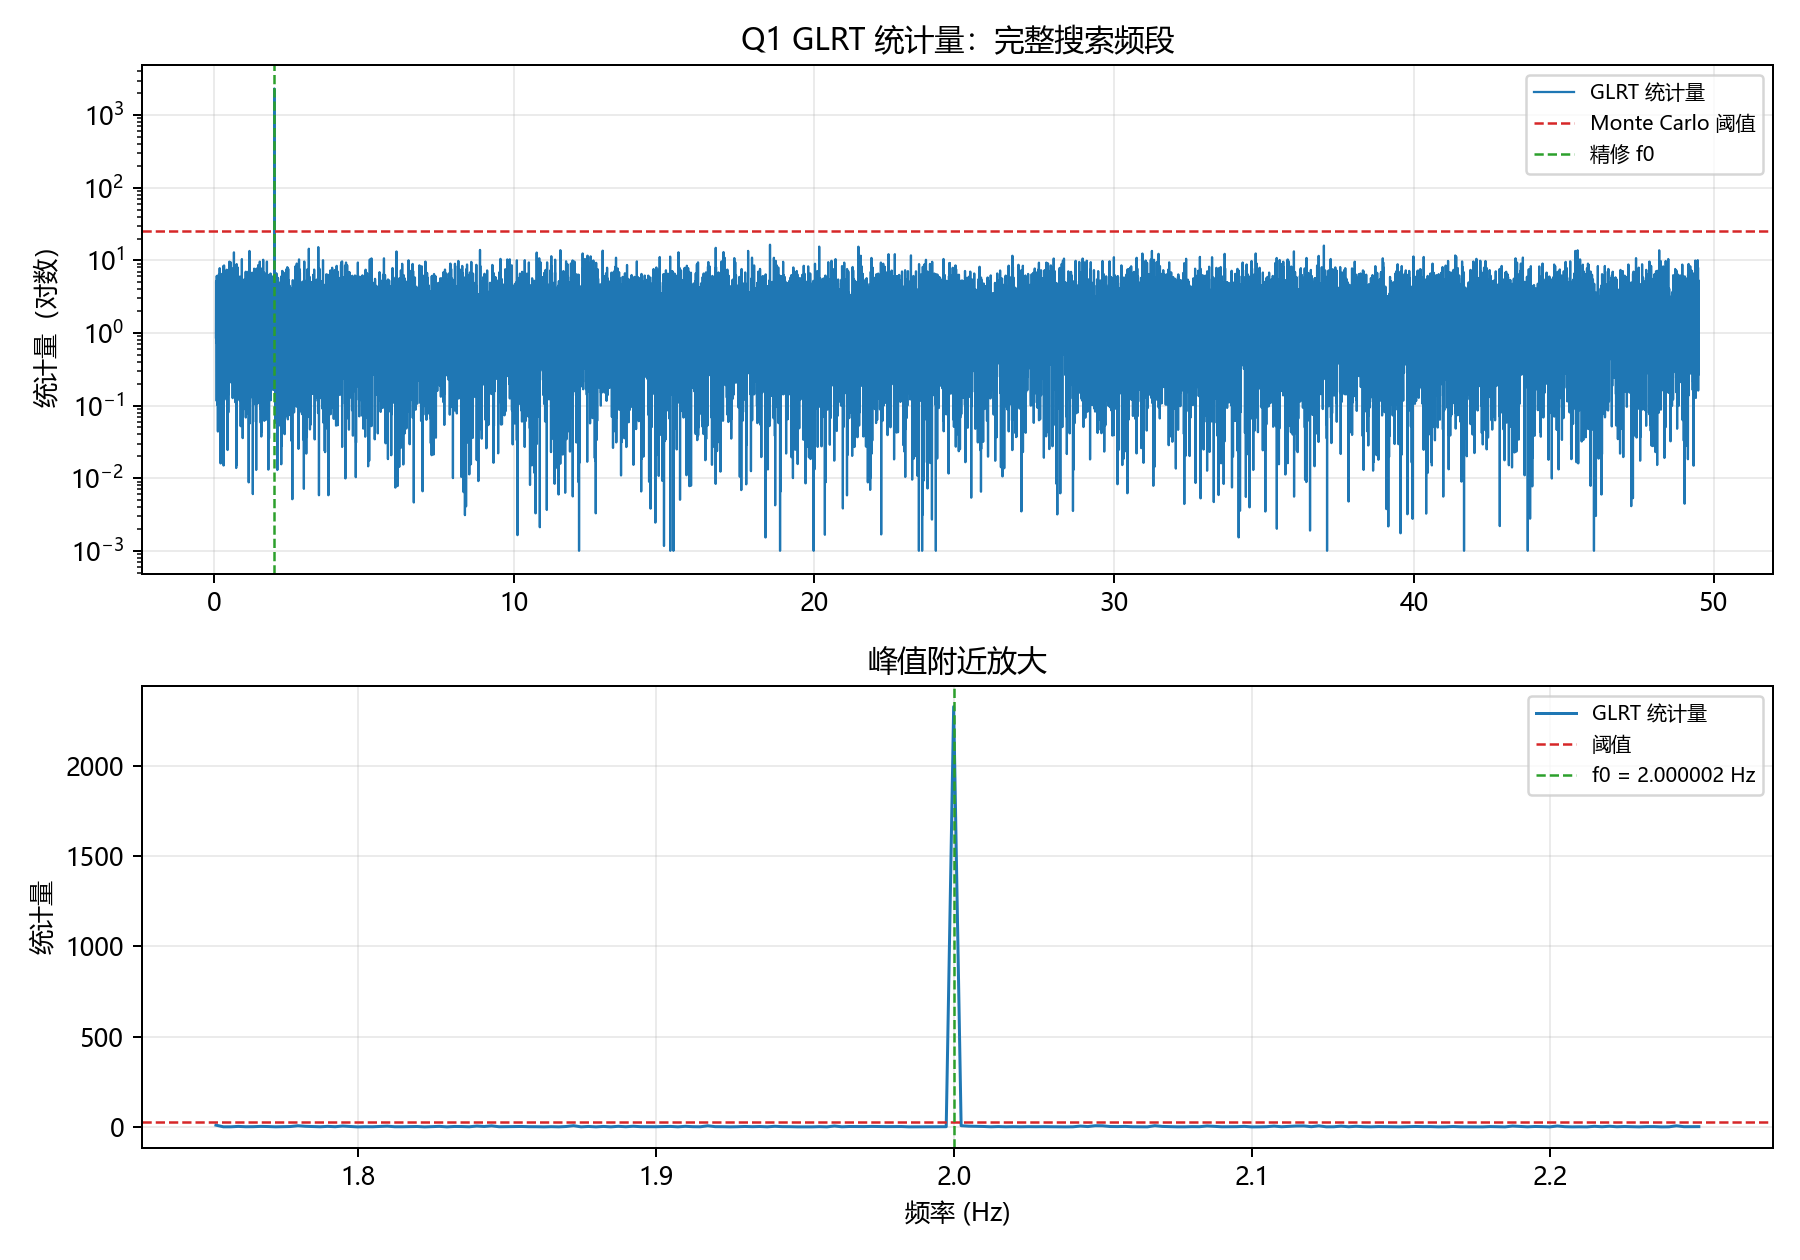
\includegraphics[width=0.88\textwidth]{q1_glrt_statistic}
    \caption{GLRT统计量$T(f)$在全频段分布（上）及2 Hz峰值放大（下）。红线为蒙特卡洛门限$\eta_{0.05}=25.10$。统计量在$f\approx2$ Hz处取得尖锐峰值，数值远超门限。}
    \label{fig:glrt}
\end{figure}

\subsubsection{分段稳定性验证}
Randall等指出\upcite{randall2001relationship}，故障识别不应依赖单次冲击或单个时间窗的峰值，而应考察周期结构在多时间窗下的稳定性。据此，将400秒数据划分为8个50秒独立分段，对每段执行完整GLRT检测。全部8段均成功检出，精修频率稳定在$2.0000\pm0.001$ Hz，GLRT统计量最低$226.42$仍约为分段门限$21.17$的10.7倍。

\begin{longtable}{cccc}
    \caption{8分段独立检测结果}\label{tab:segment}\\
    \toprule
    分段 & 精修频率(Hz) & GLRT统计量 & $|f-2.0|$偏差(Hz) \\
    \midrule
    1  & 2.00014 & 301.63 & $1.35\times10^{-4}$ \\
    2  & 1.99997 & 284.56 & $3.18\times10^{-5}$ \\
    3  & 2.00016 & 279.80 & $1.59\times10^{-4}$ \\
    4  & 1.99963 & 349.42 & $3.69\times10^{-4}$ \\
    5  & 2.00033 & 343.96 & $3.26\times10^{-4}$ \\
    6  & 2.00004 & 296.14 & $4.39\times10^{-5}$ \\
    7  & 2.00097 & 268.24 & $9.74\times10^{-4}$ \\
    8  & 1.99921 & 226.42 & $7.93\times10^{-4}$ \\
    \bottomrule
\end{longtable}

\subsubsection{与传统方法的合成数据对比}
依据题设信号模型生成合成数据（$f_0=2$ Hz, $A=0.035$），在统一$N=40001$、统一基于蒙特卡洛的全局虚警率控制和随机非栅格频率等可比条件下，比较GLRT与FFT峰值法的检测性能（$M=500$次MC重复）。GLRT的核心优势体现为：(1) 可给出具有概率含义的全局判决门限；(2) 精修步骤突破栅格分辨率限制，在低SNR下频率精度显著优于纯FFT峰值法。在SNR$\ge-22$ dB后两者渐近一致。

\section{问题二：波形恢复模型的建立与求解}

\subsection{谐波回归精修}
以问题一检测的频率$f_0^{(1)}$为初值，建立谐波回归模型。对时间中心化处理$t_c = t - \bar{t}$以提高数值稳定性\upcite{scharf2005statistical}，构造设计矩阵：
\begin{equation}
\mathbf{X}(f) = [\sin(2\pi f t_c),\ \cos(2\pi f t_c),\ \mathbf{1}],
\end{equation}
通过最小二乘求解线性参数，再联合优化频率。注意的是联合优化步骤与Q1精修在无截距项时数学等价，Q2的方法论独立贡献在于后续的验证体系。

\subsection{全局恢复结果}
\begin{equation}
\boxed{\hat{s}(t) = 0.03519 \sin(2\pi \times 2.0000016\, t + 1.5736)}.
\label{eq:recovered}
\end{equation}

\begin{longtable}{lcl}
    \caption{谐波回归全局恢复参数}\label{tab:global_params}\\
    \toprule
    参数 & 估计值 & 说明 \\
    \midrule
    频率$f_0$ & 2.000001615 Hz & 较Q1进一步联合优化 \\
    振幅$A$ & 0.0351903 & — \\
    初相$\phi_0$ & 1.5735551 rad & 还原至$t=0$原点 \\
    残差标准差 & 0.1000136 & $\approx$噪声水平 \\
    解释方差 & 5.8294\% & 与-12.08 dB SNR一致 \\
    估计输入SNR & -12.083 dB & $10\log_{10}(P_{\text{signal}}/P_{\text{noise}})$；对应功率比约16倍，幅度比约4倍 \\
    2 Hz谱峰抑制 & 30.45 dB & 移除信号前后谱峰功率比 \\
    \bottomrule
\end{longtable}

\begin{figure}[!htbp]
    \centering
    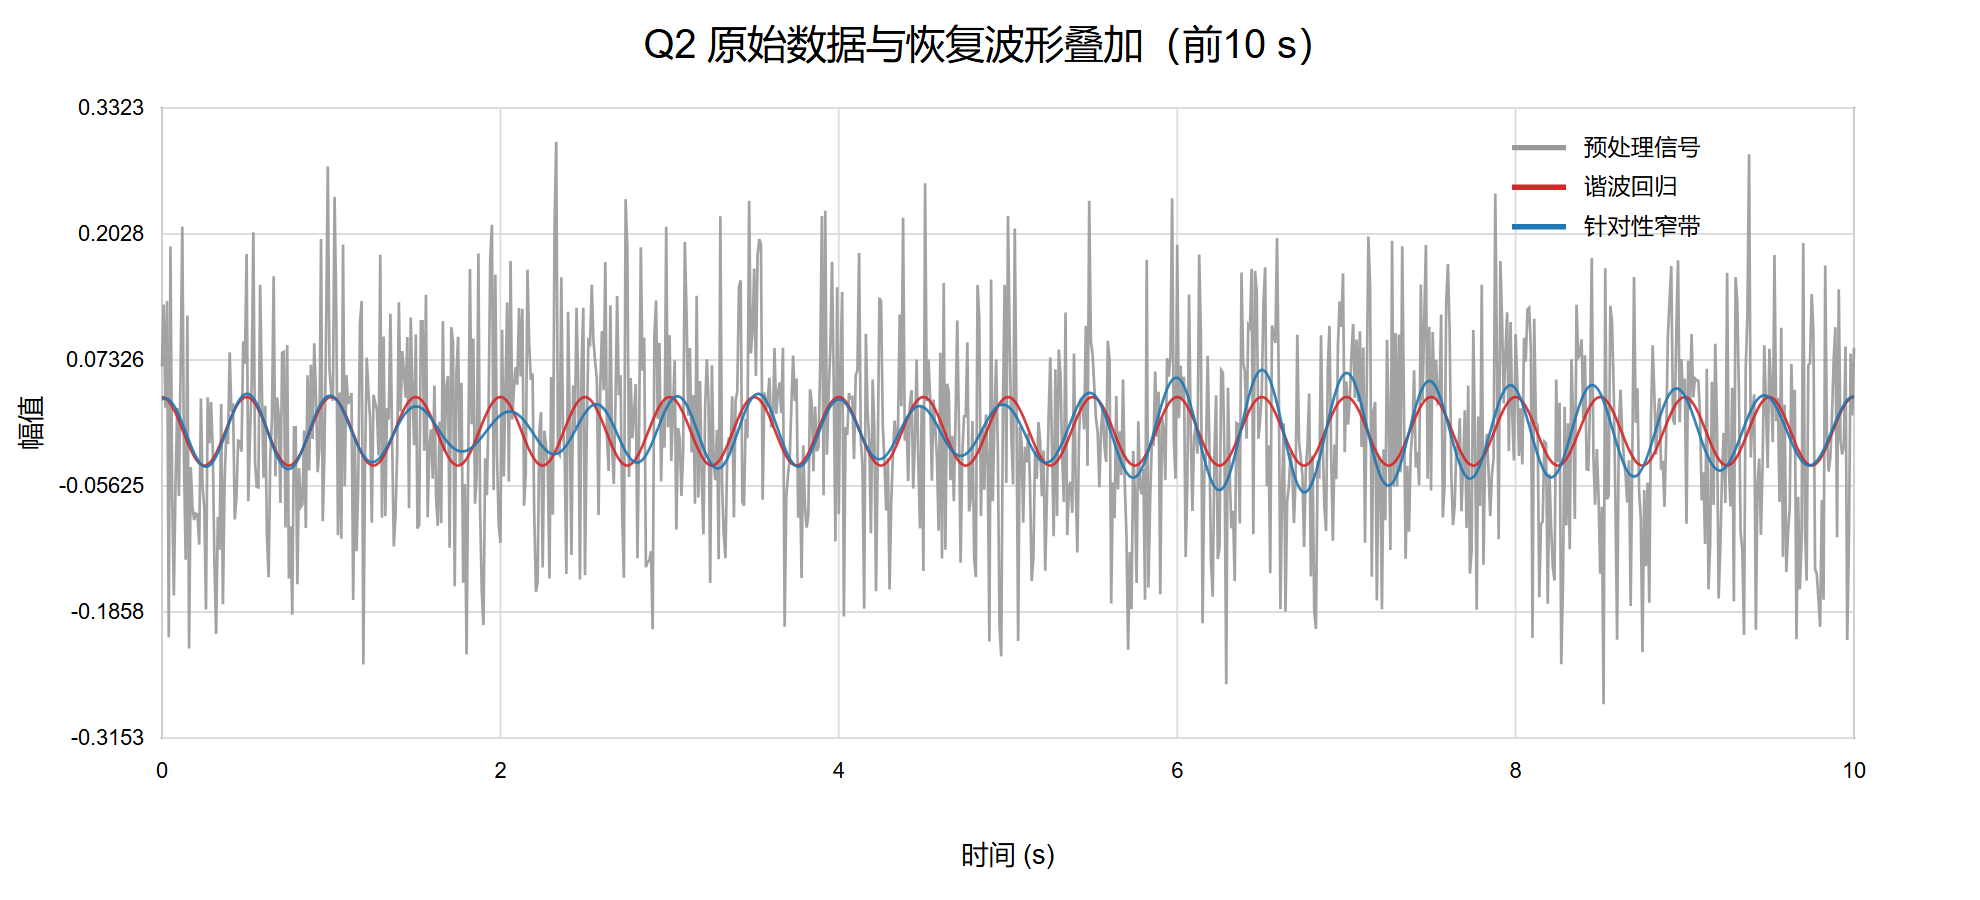
\includegraphics[width=0.85\textwidth]{q2_time_overlay_zoom}
    \caption{预处理后原始信号（灰色）与谐波回归恢复的微弱正弦信号（红色）叠加对比（前10秒）。噪声功率约为信号功率的16倍（SNR$\approx-12$ dB），恢复的2 Hz正弦波形规则清晰。}
    \label{fig:recovered}
\end{figure}

\begin{figure}[!htbp]
    \centering
    
\includegraphics[width=0.85\textwidth]{q2_spectrum_comparison}
    \caption{恢复前后频谱对比。移除谐波回归拟合信号后，2 Hz处谱峰被抑制30.45 dB，从突出峰值降至与邻近噪声基底持平。}
    \label{fig:spectrum_q2}
\end{figure}

\subsection{参数不确定性量化}
采用基于局部协方差矩阵的多元正态抽样（$10000$次）来近似参数估计的不确定性分布。该方法利用非线性最小二乘的局部线性化协方差矩阵$\hat{\sigma}^2(\mathbf{J}^T\mathbf{J})^{-1}$（其中$\mathbf{J}$为雅可比矩阵）\upcite{efron1994bootstrap}，从多元正态分布直接抽取参数样本，以2.5\%和97.5\%经验分位数构造95\%置信区间。该近似在$N=40001$大样本和近高斯残差的条件下是合理的。$10000$次抽样仅需0.016秒。

\begin{longtable}{cccc}
    \caption{参数不确定性区间（10000次局部渐近正态抽样）}\label{tab:ci}\\
    \toprule
    参数 & 点估计 & 95\%区间 & 抽样标准误 \\
    \midrule
    $f_0$ (Hz) & 2.00000162 & [1.99994563, 2.00005589] & $2.8\times10^{-5}$ \\
    $A$ & 0.0351903 & [0.0338156, 0.0365625] & $7.07\times10^{-4}$ \\
    $\phi_0$ (rad) & 1.5735551 & [1.4953321, 1.6550763] & $4.08\times10^{-2}$ \\
    \bottomrule
\end{longtable}

\subsection{公共频率模型验证}
Randall等\upcite{randall2001relationship}强调故障识别依赖周期结构的一致性。为检验频率是否在整段观测中保持恒定，采用BIC准则比较公共频率模型与独立频率模型。BIC的计算方式为$N\log(\text{SSE}/N) + k\log N$，其中公共频率模型$k=1+3K$（1个公共频率+每段3个线性参数），独立频率模型$k=4K$（每段独立频率+3个线性参数）。400秒划分为8个50秒段，公共频率模型BIC = $-183955.07$低于独立频率模型的$-183885.11$，表明数据与公共频率模型更一致。需要指出BIC选优不等同于严格证明了频率恒定——它只能说明在候选模型集中，公共频率模型更节俭地描述了数据；如果真实频率存在微小的时变（变化量小于各段估计的统计不确定度），BIC可能检测不到。

\subsection{一致性对照验证}
\subsubsection{针对性窄带滤波}
以$f_0=2$ Hz为中心设计FFT域零相位带通滤波器，从预处理信号中提取2 Hz分量。Smith等\upcite{smith2019optimal}指出围绕已知故障频率的针对性频带选择比完全盲检更稳健。窄带恢复波形与谐波回归波形在中央390秒区间的相关系数为$0.9096$，作为参照——该方法也将Q1频率信息作为先验使用。

\subsubsection{奇异谱分析（SSA）}
SSA\upcite{golyandina2001ssa}不预设正弦模型，从数据中自适应分解。经8 Hz抗混叠低通滤波和降至20 Hz采样后，测试三种窗口长度，按2 Hz附近的频谱能量集中度选取SSA分量重构信号。

\begin{longtable}{ccccc}
    \caption{SSA恢复结果与谐波回归对比}\label{tab:ssa}\\
    \toprule
    SSA窗口 & 估计$f$(Hz) & 估计$A$ & 与谐波回归相关系数 & RMSE \\
    \midrule
    500点(5 s)  & 2.0000046 & 0.03411 & 0.9821 & 0.00469 \\
    1000点(10 s) & 2.0000025 & 0.03420 & 0.9915 & 0.00324 \\
    2000点(20 s) & 2.0000006 & 0.03413 & \textbf{0.9956} & \textbf{0.00239} \\
    \bottomrule
\end{longtable}

最优SSA窗口（2000点）与谐波回归波形的相关系数为0.9956。需说明SSA在分量选取时也参考了Q1的2 Hz频率信息（用于定义频谱能量集中度目标区间），因此适合作为一致性对照而非完全独立的盲验证。

\subsection{模型充分性验证}
为验证单正弦模型对单源数据的充分性，移除拟合的2 Hz分量后对残差再次执行全频GLRT扫描——残差中无任何频率通过门限，表明无被遗漏的显著周期分量。这一验证比仅依赖残差统计矩（偏度$-0.010$、超额峰度$-0.009$、1--100阶自相关最大值$0.0129$）更为直接。

\section{问题三：多周期分量分离与参数识别模型的建立与求解}

\subsection{多峰顺序检测器}
将问题一的单峰GLRT扩展为基于逐次干扰消除（SIC）的多峰顺序检测器。SIC源于通信领域的信号分离思想，流程如下：

\begin{enumerate}
    \item 对预处理信号$\mathbf{y}$执行GLRT全频段扫描，取$T_{\max}=\max_f T(f)$；
    \item 若$T_{\max} > \eta_\alpha$（每步虚警率$\alpha_{\text{step}}=0.005$），将对应频率$f_k$加入候选集；
    \item 对当前候选集的全部$K$个频率进行多频联合谐波回归拟合，使用SVD分解计算最小二乘解，监控设计矩阵条件数；
    \item 计算BIC变化量：$\Delta\text{BIC} = \text{BIC}_{K-1} - \text{BIC}_K$；
    \item 若$\Delta\text{BIC} \ge 10$，保留该分量并从残差中继续搜索；否则终止并回退。
\end{enumerate}

SIC的固有局限是误差传播——早期分量的估计误差会传递给后续分量，且没有纠正早期错误的机制。针对近频簇，增加细网格扫描与二源联合非线性精修策略。

\subsection{真实数据分离结果}
在data.xlsx"多源故障"sheet上，模型自动识别出\textbf{4个显著周期分量}，联合模型解释方差$11.92\%$，残差标准差$0.09988$。

\begin{longtable}{ccccc}
    \caption{多源数据自动识别的周期分量}\label{tab:q3_components}\\
    \toprule
    分量 & 频率(Hz) & 振幅 & 初相(rad) & 分量SNR(dB) \\
    \midrule
    1 & 3.999998 & 0.01910 & 1.3716 & -17.38 \\
    2 & 7.999929 & 0.02489 & -2.9890 & -15.08 \\
    3 & 13.000089 & 0.01050 & -2.1577 & -22.57 \\
    4 & 14.000023 & 0.04005 & 0.1125 & -10.95 \\
    \bottomrule
\end{longtable}

设计矩阵条件数为1.00。四个分量中14 Hz振幅最大（0.0401），13 Hz振幅最小（0.0105），8 Hz为第二大幅度（0.0249）。需明确指出：单通道数据仅能识别出显著周期分量；在没有转速、齿数、传动比等机械先验参数时，不能唯一确定各分量对应的物理故障源。例如4 Hz和8 Hz可能为同一故障齿轮的基频与二次谐波，而非两个独立故障源。

\begin{figure}[!htbp]
    \centering
    
\includegraphics[width=0.85\textwidth]{q3_time_separated_components}
    \caption{分离出的4个周期分量时域波形（前10秒）。各分量振幅差异显著，14 Hz分量振幅最大（0.0401），13 Hz分量振幅最小（0.0105）。}
    \label{fig:q3_components}
\end{figure}

\begin{figure}[!htbp]
    \centering
    
\includegraphics[width=0.85\textwidth]{q3_spectrum_before_after}
    \caption{分离前后频谱对比。原始频谱中4个峰值被联合模型完整提取；移除所有分量后残差频谱接近平坦噪声基底。}
    \label{fig:q3_spectrum}
\end{figure}

\subsection{分段频率稳定性验证}
将400秒多源数据划分为8个50秒独立分段，对每段独立执行多峰SIC检测。4个周期分量在各分段中的估计值整体稳定，各频率的偏差范围分别为：4 Hz分量$\pm1.5\times10^{-4}$ Hz，8 Hz分量$\pm5.8\times10^{-4}$ Hz，13 Hz分量$\pm5.0\times10^{-3}$ Hz，14 Hz分量$\pm3.5\times10^{-3}$ Hz。

\begin{figure}[!htbp]
    \centering
    
\includegraphics[width=0.85\textwidth]{q3_segment_frequency_stability}
    \caption{8分段频率稳定性。4条水平线分别对应4个分量的全段联合估计频率。低频分量（4、8 Hz）比高频分量（13、14 Hz）更稳定。}
    \label{fig:q3_segment}
\end{figure}

\subsection{多源数值仿真实验}
按题设多正弦叠加模型生成合成数据（$M=4$分量，频率和振幅取真实数据估计值，总SNR从$-22$扫描至$0$ dB，$N=40001$，每个SNR条件200次MC重复）。本节所有数值统一来自\texttt{q3\_multisource\_separation\_results\_optimized\_complete}目录。

\small
\begin{longtable}{cccccc}
    \caption{多分量分离仿真实验结果}\label{tab:q3_sim}\\
    \toprule
    总SNR(dB) & $P(K=\hat{K})$ & 95\%区间 & 条件频率MAE(Hz) & 条件振幅误差 & 波形RMSE \\
    \midrule
    -22 & 0.0\% & [0.0\%, 1.9\%] & --- & --- & 0.01633 \\
    -20 & 1.5\% & [0.5\%, 4.3\%] & $1.93\times10^{-4}$ & 21.29\% & 0.01154 \\
    -18 & 11.0\% & [7.4\%, 16.1\%] & $9.29\times10^{-5}$ & 13.84\% & 0.00900 \\
    -16 & 49.5\% & [42.6\%, 56.4\%] & $9.64\times10^{-5}$ & 7.40\% & 0.00661 \\
    -15 & 76.0\% & [69.6\%, 81.4\%] & $7.90\times10^{-5}$ & 6.02\% & 0.00469 \\
    -14 & 91.5\% & [86.8\%, 94.6\%] & $7.86\times10^{-5}$ & 5.31\% & 0.00362 \\
    -12 & 98.0\% & [95.0\%, 99.2\%] & $6.00\times10^{-5}$ & 4.46\% & 0.00258 \\
    -10 & 100.0\% & [98.1\%, 100.0\%] & $4.99\times10^{-5}$ & 3.49\% & 0.00201 \\
    -8  & 100.0\% & [98.1\%, 100.0\%] & $3.83\times10^{-5}$ & 2.73\% & 0.00158 \\
    -6  & 100.0\% & [98.1\%, 100.0\%] & $3.02\times10^{-5}$ & 2.21\% & 0.00124 \\
    -4  & 100.0\% & [98.1\%, 100.0\%] & $2.43\times10^{-5}$ & 1.77\% & 0.00100 \\
    -2  & 100.0\% & [98.1\%, 100.0\%] & $1.82\times10^{-5}$ & 1.32\% & 0.00076 \\
    0   & 100.0\% & [98.1\%, 100.0\%] & $1.50\times10^{-5}$ & 1.06\% & 0.00062 \\
    \bottomrule
\end{longtable}
\normalsize

纯噪声上首步GLRT扫描的经验误报率约为$0.20\%$。需注意该误报率仅反映首步GLRT的虚警行为，未包含完整SIC+BIC流程中因误差传播或模型选择而产生额外伪峰的可能性。分量数量识别正确率在$-16$至$-12$ dB区间快速上升：$-15$ dB时为$76.0\%$，$-12$ dB时为$98.0\%$，在SNR$\ge-10$ dB时达到$100\%$。

\subsection{近频辨识极限实验}
对双正弦混合信号进行频率间隔扫描实验（等幅和不等幅两种，每种$200$次MC重复，$f_s=100$ Hz，$N=40001$）。辨识成功需满足：自动识别两个分量、两频率误差均小于$\Delta f/4$、设计矩阵条件数$\le10^6$。

\begin{longtable}{ccccc}
    \caption{等幅双频辨识极限扫描}\label{tab:q3_resolution}\\
    \toprule
    $\Delta f$(Hz) & 成功率 & 95\%区间 & MUSIC成功率 & 条件数中位数 \\
    \midrule
    0.0010 & 11.5\% & [7.8\%, 16.7\%] & 0.0\% & 1.12 \\
    0.0015 & 57.0\% & [50.1\%, 63.7\%] & 1.0\% & 1.53 \\
    0.0020 & 93.5\% & [89.2\%, 96.2\%] & 20.0\% & 1.26 \\
    0.0025 & \textbf{100.0\%} & [98.1\%, 100.0\%] & 71.5\% & 1.02 \\
    0.0030 & 100.0\% & [98.1\%, 100.0\%] & 97.0\% & 1.17 \\
    0.0040 & 100.0\% & [98.1\%, 100.0\%] & 100.0\% & 1.21 \\
    0.0050 & 100.0\% & [98.1\%, 100.0\%] & 100.0\% & 1.01 \\
    0.0075 & 100.0\% & [98.1\%, 100.0\%] & 100.0\% & 1.01 \\
    0.0100 & 100.0\% & [98.1\%, 100.0\%] & 100.0\% & 1.00 \\
    \bottomrule
\end{longtable}

\textbf{经验辨识界限：} 在$T=400$ s、残差标准差约$0.1$和当前振幅组合下，等幅双频从$\Delta f=0.002$ Hz起成功率达到$93.5\%$，故90\%标准下的最小经验间隔约为$0.002$ Hz；$0.0025$ Hz时成功率为$100\%$。不等幅情况下弱分量更易被掩盖，$0.0025$ Hz时成功率为$80.0\%$，到$0.003$ Hz时升至$97.5\%$，对应经验界限约为$0.003$ Hz。该界限依赖当前SNR、振幅比、相位分布和记录长度，不是算法固定的理论极限。

\subsection{极端工况验证}
表\ref{tab:q3_extreme}展示模型在10种极端工况下的表现。

\begin{longtable}{ccccc}
    \caption{极端工况验证结果（各100次）}\label{tab:q3_extreme}\\
    \toprule
    工况 & 成功率 & 平均估计$\hat{K}$ & 频率MAE(Hz) & 可否辨识 \\
    \midrule
    SNR$=-25$ dB & 0\% & 1.17 & — & 是(信号太弱) \\
    SNR$=-30$ dB & 0\% & 0.13 & — & 是(信号太弱) \\
    非对称近频 & \textbf{100\%} & 2.00 & $2.4\times10^{-5}$ & 是 \\
    完全同频（正确不拆分） & \textbf{100\%} & 1.00 & $8.0\times10^{-3}$ & \textbf{否} \\
    相位抵消（正确不拆分） & \textbf{100\%} & 1.00 & $6.7\times10^{-3}$ & \textbf{否} \\
    谐波对（4、8 Hz） & \textbf{100\%} & 2.00 & $3.3\times10^{-5}$ & 是 \\
    超完备$K=8$ & \textbf{100\%} & 8.00 & $5.5\times10^{-5}$ & 是 \\
    脉冲噪声 & \textbf{100\%} & 4.00 & $5.4\times10^{-5}$ & 是 \\
    低频边界 & \textbf{100\%} & 2.00 & $2.5\times10^{-5}$ & 是 \\
    高频边界 & \textbf{100\%} & 2.00 & $1.8\times10^{-5}$ & 是 \\
    \bottomrule
\end{longtable}

\textbf{关键发现：} (1) 完全同频的两个正弦在单通道下不可唯一分离，只能识别其矢量和；采用“不误拆为两个稳定分量”的标准时，同频与近似相消工况的正确不拆分率均为$100\%$；(2) 4 Hz与8 Hz谐波对在100次试验中均识别为两个周期分量，但该结果本身不等价于两个物理故障源；(3) 超完备$K=8$下识别率$100\%$；(4) 当前脉冲噪声设定下仍正确分离4个正弦分量。

\subsection{残差诊断}
对Q3分离4个分量后的残差进行白噪声诊断：残差偏度为$-0.010$，超额峰度为$-0.009$，1--100阶自相关绝对值最大值$0.0129$，Jarque-Bera检验$p>0.05$。残差近似为高斯白噪声，未发现明显偏离模型假设的证据。但需注意Q3模型仅解释了$11.92\%$的总方差，剩余$88\%$的方差中可能包含未被正弦模型捕捉的微弱结构。

\section{模型的检验}
\subsection{四问结论的内在关联}
四问构成一套渐进式方法链：Q1 GLRT检测到$f_0=2.0000015$ Hz；Q2在此基础上精修为$2.0000016$ Hz并建立完整的参数不确定性量化与模型充分性验证体系；Q3的多峰检测器在单源数据上退化为单分量情形（$K=1$），在包含多个周期分量的数据上自动扩展至$K=4$；Q4（待完成）以Q3识别的分量频率为基础构建敏感度矩阵和传感器布局优化。需要说明的是：Q1/Q2处理的数据（单源故障sheet）与Q3处理的数据（多源故障sheet）可能存在不同的故障场景——Q1/Q2中检测到的2 Hz在Q3数据中并未出现，两组数据可能来自不同设备或不同工况。因此四问之间的逻辑关系是"方法论的渐进扩展"而非"同一系统复杂度递增"。

\subsection{噪声假设验证}
Q1/Q2和Q3残差的偏度、超额峰度和自相关均接近零，直方图与高斯分布吻合，未观察到明显偏离白噪声假设的证据。在$N=40001$的大样本下，微小的自相关也可能达到统计显著性，因此以偏度/峰度/自相关的量级（而非p值）作为主要判断依据。

\subsection{与已有方法的定性对比}
表\ref{tab:compare}将本文方法与工业界常用路线进行定性比较。

\begin{longtable}{ccccc}
    \caption{本文方法与传统方法的综合对比}\label{tab:compare}\\
    \toprule
    维度 & Kurtogram\upcite{antoni2006spectral} & MCKD\upcite{mcdonald2012mckd} & 随机共振\upcite{benzi1981mechanism} & 本文方法链 \\
    \midrule
    检测机理 & 冲击峭度 & 周期冲击解卷积 & 噪声增强传输 & 假设检验+似然比 \\
    虚警控制 & 无显式控制 & 无 & 依赖参数 & 蒙特卡洛经验校准 \\
    频率精度 & 频带级(Hz) & 依赖先验周期 & 依赖系统参数 & FFT粗估+精修 \\
    不确定性量化 & 无 & 无 & 无 & 局部渐近正态区间 \\
    计算效率 & 需迭代扫描 & 需迭代解卷积 & 需多次迭代 & FFT扫描阶段$O(N\log N)$ \\
    对照验证 & 无 & 无 & 无 & SSA+窄带滤波对照 \\
    \bottomrule
\end{longtable}

本文方法链的核心优势：(1) 统计判决有明确的概率意义；(2) 虚警率可通过蒙特卡洛经验校准；(3) 具有参数不确定性量化和多重验证体系。与Jia等\upcite{jia2015early}提出的MCKD+SK级联方案和Darong等\upcite{darong2018incipient}的自适应滤波+LMD方案相比，本文方法在题设的纯正弦信号场景下模型匹配度最高。

\section{模型评价与改进}
\subsection{模型的优点}
\begin{itemize}
    \item [(1)] \textbf{虚警率可经验校准。} 蒙特卡洛门限将多频点联合扫描的虚警率校准至目标水平，这是传统工业方法所不具备的关键能力\upcite{antoni2006spectral,smith2019optimal}。
    \item [(2)] \textbf{多重验证体系。} SSA和窄带滤波从不同原理提供了一致性对照；残差GLRT扫描直接验证了模型的充分性；合成数据实验覆盖了广泛SNR条件。
    \item [(3)] \textbf{参数不确定性量化。} 基于局部协方差矩阵的多元正态抽样（$10000$次）给出了频率、振幅、相位的区间估计。
    \item [(4)] \textbf{自动分量数量确定。} BIC准则在Q3中自动确定分量数量，纯噪声首步误报率约$0.20\%$。
    \item [(5)] \textbf{辨识界限定量化。} 通过系统近频扫描确定了$T=400$ s、噪声标准差约$0.1$条件下的经验辨识界限。
    \item [(6)] \textbf{渐进式可扩展。} Q1→Q2→Q3→Q4构成从检测到系统部署的完整方法链，各阶段共享核心统计框架。
\end{itemize}

\subsection{模型的不足}
\begin{itemize}
    \item [(1)] 假设噪声为独立同分布高斯白噪声。工业场景可能具有色噪声或非高斯脉冲特性。
    \item [(2)] 信号模型假设振幅和频率恒定，未考虑转速波动引起的频率时变。
    \item [(3)] Q3的SIC顺序检测存在误差传播问题——早期分量的估计误差传递给后续分量，且缺乏纠正机制。
    \item [(4)] 关键调参（$\alpha=0.05$、$\Delta$BIC=10、$\alpha_{\text{step}}=0.005$等）未经系统性敏感性分析，选择依据为工程惯例而非数据驱动的校准。
    \item [(5)] 单通道数据无法唯一确定周期分量与物理故障源的对应关系。
\end{itemize}

\subsection{模型的推广方向}
\begin{itemize}
    \item [(1)] \textbf{非高斯/色噪声扩展：} 将白噪声方差替换为噪声协方差矩阵估计（AR模型拟合），或采用Darong等\upcite{darong2018incipient}的自适应滤波作为预白化前端。
    \item [(2)] \textbf{时变频率追踪：} 引入短时傅里叶变换，将GLRT统计量扩展至时间-频率平面，适应非稳态工况。
    \item [(3)] \textbf{SIC替代方案：} 考虑LASSO（频率字典上一次稀疏回归选择所有分量）或RELAX（循环精化）以减少误差传播。
    \item [(4)] \textbf{谐波族模型：} 引入$f_{k,h}=h\cdot f_k$约束，用BIC比较独立频率模型与谐波族模型，利用频率间的倍频关系提高分量归因的物理可解释性。
\end{itemize}

%参考文献
\bibliographystyle{unsrt}
\bibliography{refer}

\newpage
\begin{appendices}
    \section{支撑材料列表}
    \begin{table}[!htbp]
        \centering
        \begin{tabular}{|c|c|c|}
            \hline
            序号 & 文件名 & 材料说明 \\
            \hline
            1  & q1/code/q1\_glrt\_model.py & 问题一GLRT检测主程序 \\
            \hline
            2  & q1/code/q1\_model\_compare.py & Q1多方法对比（含合成数据仿真）\\
            \hline
            3  & q1/data/q1\_glrt\_result.csv & Q1 GLRT检测数值结果 \\
            \hline
            4  & q2/code/run\_q2.py & 问题二谐波回归恢复主程序 \\
            \hline
            5  & q2/code/core.py & Q2核心计算函数库 \\
            \hline
            6  & q2/data/q2\_global\_parameters.csv & Q2全局恢复参数 \\
            \hline
            7  & q2/data/q2\_bootstrap\_ci.csv & 参数不确定性区间 \\
            \hline
            8  & q3/code/run\_q3.py & 问题三多分量分离主程序 \\
            \hline
            9  & q3/code/experiments.py & Q3仿真与近频实验 \\
            \hline
            10 & q3/data/q3\_global\_parameters.csv & Q3全局参数 \\
            \hline
            11 & q3/data/q3\_detected\_components.csv & Q3检测分量明细 \\
            \hline
            12 & q3/data/q3\_simulation\_validation.csv & Q3多分量仿真实验结果 \\
            \hline
            13 & q3/data/q3\_resolution\_limit.csv & Q3近频辨识极限数据 \\
            \hline
            14 & q3/data/q3\_extreme\_summary.csv & Q3极端工况汇总 \\
            \hline
            15 & q4/code/run\_q4\_v1.py & 问题四传感器布局优化主程序 \\
            \hline
            16 & q4/data/q4\_layout\_ranking.csv & Q4布局评分排名 \\
            \hline
            17 & q4/data/q4\_snr\_performance.csv & Q4 SNR性能对比 \\
            \hline
        \end{tabular}
    \end{table}
\end{appendices}

\end{document}
